\documentclass[10.5pt, a4paper, twoside]{article}
\providecommand{\abs}[1]{\lvert#1\rvert}
\setlength{\topmargin}{-1.25in}
\setlength{\footskip}{0.75in}
\setlength{\textheight}{10in}

\usepackage[margin=2.5cm]{geometry}
\usepackage{amsfonts}
\usepackage{amsmath}
\usepackage{amssymb}
\usepackage{graphicx}
\usepackage{enumerate}
\usepackage{color}
\usepackage{setspace}
\usepackage{tabularx}
\setlength{\extrarowheight}{5pt}
\usepackage[labelfont=bf]{caption}
\usepackage{subfig}

%%%% BIBLIO

\usepackage[backend=bibtex]{biblatex}

%%%% GLOSSARY STUFF

\usepackage[intoc]{nomencl} 

\renewcommand{\nomname}{Glossary}
\renewcommand{\nomlabel}[1]{\textbf{#1}}
\makenomenclature

%\singlespacing
\onehalfspacing
%\doublespacing
%\setstretch{1.1}

\setlength\parindent{0pt}

\newenvironment{packed_itemize}{
\begin{itemize}
  \setlength{\itemsep}{1pt}
  \setlength{\parskip}{0pt}
  \setlength{\parsep}{0pt}
}{\end{itemize}}

\definecolor{dkgreen}{rgb}{0,0.6,0}
\definecolor{gray}{rgb}{0.5,0.5,0.5}
\definecolor{mauve}{rgb}{0.58,0,0.82}

\newcommand{\vecthree}[3]{\left(\!\!{\scriptsize\begin{array}{c}#1\\#2\\#3\end{array}}\!\!\right)}
\newcommand{\vectwo}[3]{\left(\!\!{\scriptsize\begin{array}{c}#1\\#2\end{array}}\!\!\right)}
\newcommand{\HRule}{\rule{\linewidth}{0.5mm}}

\newcolumntype{C}{>{\centering\arraybackslash}X}
\newcolumntype{L}{>{\raggedright\arraybackslash}X} 

\addbibresource{sources.bib}

\begin{document}
%
%\title{ \bf \huge Development of a 12.4 GHz Bandwidth Frequency Offset Locking Unit for Two-Laser Systems}
%\author{Steve Novakov }
%\date{}
%
%\maketitle

\begin{titlepage}
\begin{center}

% Upper part of the page. The '~' is needed because \\
% only works if a paragraph has started.

% Title
\HRule \\[0.4cm]
{ \huge \bfseries Pound-Drever-Hall Servomechanism with an Atomic Referece for Frequency Stabilization of a Master Laser \\[0.4cm] }

\HRule \\[2.5cm]

% Author and supervisor

\begin{tabularx}{\linewidth}{lXr}
  \Large \emph{Authors:} & & \Large \emph{Sponsor:} \\
  \Large \textsc{Steve Novakov} & & \Large \textsc{Dr.~Kirk Madison} \\
  \Large \textsc{Jeff Taylor}  & & \\
\end{tabularx}

\vfill

\textsc{\LARGE ENPH 479}\\[0.3cm]
\textsc{\LARGE Engineering Physics}\\[0.3cm]
\textsc{\LARGE University of British Columbia}\\[0.3cm]

\vfill

\textsc{\Large Group 1472}\\[0.3cm]
\textsc{\Large Project 33}\\[0.3cm]

\vfill

% Bottom of the page
{\large \today}

\end{center}
\end{titlepage}
\newpage

%%%%%%%%%%%%%%%% EXECUTIVE SUMMARY

\newpage
\section*{Executive Summary}

This project, sponsored by the UBC Quantum Degenerate Gases
Laboratory - Madison Group, aims to build and characterize a high
fidelity, small linewidth, laser frequency locking system based on the
Pound-Drever-Hall (PDH) locking method. The QDG laboratory 
specializes in manipulation of atomic and molecular gases with
optical systems that implement some form of laser cooling. To 
efficiently cool or manipulate these ensembles, the lasers involved
must be tuned to specific frequencies, often corresponding to atomic
transitions, and have as small a linewidth as possible. Any increase 
in the fidelity of the probing or pumping lasers often has immediate
impact on the quantity of atoms that can be trapped/cooled, and the 
lowest attainable temperature in a trap. Specifically, in some cases, 
the linewidth must be as small as possible around the resonant frequency 
of a transition. \\

Existing systems at the sponsors' laboratory are already based 
on the PDH method, but use a slightly different approach. Both the 
existing and proposed systems will lock to a frequency-discriminating 
object, specifically a vapor cell of the relevant atomic species. The
existing locking unit makes use of an Acousto-optic Modulator (AOM), a 
device which takes a seeding beam from a diode laser as an input and, 
through acoustic vibration generated by a piezo-electric transducer, 
produces a Doppler-shifted diffraction pattern. This pattern is then 
sent through a vapor cell (though commonly, an external cavity is used), 
and the filtered beam is coupled into a photosensor and mixed/processed 
to produce an error signal. This signal is then used by the diode laser 
control system to lock to the resonance frequency of the selective 
element. Unfortunately, due to mechanical limitations of the AOM device, 
the dithering frequency of the modulated beam output, which drives the 
resolution of the error signal, is quite small, approximately 200 kHz. 
Furthermore, the processing required to use this signal decreases the 
settling time further, approximately 10-20 fold to 10 kHz [maybe cite 
something here, rather than relying on just Kirk's description]. This 
results in a large setting time for the control circuit, which 
necessarily increases the linewidth of the laser.  \\

To increase the bandwidth of the locking circuit and therefore 
reduce the linewidth of the master laser, a PDH unit based around an 
Electro-Optic Modulator (EOM) will be built, and its performance will be 
benchmarked to the existing AOM locking unit. An EOM, commonly known as 
a "Pockels Cell" as it exploits the Pockels Effect, is a physical medium 
which phase modulates a beam in its direction of propagation at a 
driving frequency. The output beam has the same fundamental as the input 
beam, as well as a well-defined spectrum of side-bands. This composite 
beam is then sent through the frequency selective unit and, again, mixed 
to produce an error signal. The primary difference, relative to the AOM 
unit, is that the mixing technique is slightly different and, more 
importantly, that the dithering frequency is significantly higher. Some 
EOM units can handle modulation at over 100 MHz, though, for this 
project, a frequency of 10-20 MHz will likely be sufficient. This 
drastic increase in the control loop bandwidth will result in a much 
smaller linewidth for the master laser, and, ultimately, higher 
experimental efficiency. \\

There will be three primary stages to this project. First, the 
existing system will be evaluated for key parameters such as laser 
linewidth, and the relationships between factors like the noise floor,
modulation frequency and the transfer function of the frequency selective
unit will be quantified and recorded as benchmarks. This information 
will be used to spec various optical and electronic components for the
locking unit. Second, the locking unit will be designed to fit on an 
optical breadboard of convenient size. It is possible that a custom CCA 
will have to be designed to control the EOM, generate the error signal, 
and interface with laboratory computers. Third, the built locking unit 
will be tested and benchmarked against the metrics obtained from the 
existing setup. The target linewidth of the master laser will be determined during the first design stage.
 


%%%%%%%%%%%%%%%% TOC / FIGURES / TABLES
\newpage
\tableofcontents
\newpage
\listoffigures
\listoftables

%%%%%%%%%%%%%%% GLOSSARY

\newpage
\section*{Glossary}

\begin{tabularx}{\linewidth}{lX}
  {\bf CCA} & Circuit Card Assembly: includes a PBC and all of its components,
  sometimes encludes complimentary mechanical components as well. \\
  {\bf DDS} & Direct digital synthesizer: a synthesizer used for creating
  arbitrary waveforms from a reference clock. \\
  {\bf EMI} & Electromagnetic Interference: two types: radiated and conducted.\\
  {\bf FO (Receiver)} & Fiber Optic (photosensor unit for detecting fiber optic
  signals).  \\
  {\bf MOT} & Magneto-optical Trap. \\
  {\bf PCB} & Printed Circuit Board. \\
  {\bf PSU} & Power supply unit. \\
  {\bf RF} & Radio Frequency. Used to refer to components or systems which
  operate in the 3 kHz - 300 GHz regime. \\
  {\bf ROSA} & Receiver optical sub-assembly \\
  {\bf SMPS} & Switch-mode Power Supply: a power supply that utilizes
  energy conversion principles such as buck, boost, buck-boost, etc, typically
  driven at a particular switching frequency, as per the demands of the
  application. \\
  {\bf VCO} & Voltage Controlled Oscillator, may be crystal or PLL based. \\
  {\bf $V_{PP}$} & Peak-to-peak voltage: the full range of voltage of a
  particular waveform.
\end{tabularx}

%%%%%%%%%%%%%%%% BACKGROUND/MOTIVATION/OBJECTIVES

\newpage
\section{Introduction}

\subsection{Laser Locking}

The ability to lock a laser to a very specific frequency is of great importance to the UBC Quantum Degenerate Gases Laboratory.  They use these optical systems to laser cool atomic and molecular gases.  This requires a very narrow linewidth on the laser, and a specific frequency.  Any improvement in the frequency precision of the laser will increase the quantity of atoms that can be trapped or cooled, as well as the attainable temperatures in a trap.  Often, this frequency must be very close to the natural transitions of the gas.

One way to acquire such a system is to pass the beam through a gas.  The gas has transitions at particular energies, which can be detected by sweeping the laser (or an associated probe beam).  When doing this, the gas atoms will absorb photons at the corresponding frequencies, which will appear on a spectrum analyser.  However, since the gas is at room temperature, the broad absorption dip will have a bandwidth of about 1GHz, which is too wide to lock a laser to.

\subsection{Doppler Effects}

Since the gas atoms are moving in different directions, some atoms will be moving towards the laser beam, and other atoms will be moving away from it (some will be in between, of course).  As a result, if a single laser is used, the atoms moving towards the laser will perceive a higher frequency, and thus will excite at lower frequencies than the resonance frequency.  The opposite is also true.  If the absorption-vs-frequency curve is measured for a laser passed through the gas, there is a wide smear that is approximately 1GHz wide \cite{madison14}.  This makes the apparent spectrum of the gas much wider, and thus, much harder to lock a signal to.  This is depicted in Figure~\ref{fig:doppler}.

A major improvement is to redirect the single frequency laser around the sample, to the opposite side.  Now, when the sweep laser is at the same frequency as the pumping laser, its light will not be absorbed by the atoms with zero horizontal velocity.  This creates a Doppler-cancelled feature, which is about 10--100MHz wide.

\subsection{Acousto-Optic Modulator}

One way to modulate the frequency of the beam is to use an *acousto-optic modulator* (AOM).  An AOM is a device that acoustically varies its shape, adjusting the distance the light has to travel to reach its destination.  By modulating this at a frequency $\Omega$, we produce a beam of light with sidebands at $\omega + \Omega$ and $\omega - \Omega$, where $\omega$ is the original frequency of the laser. These devices use acoustics, so they are limited by the mechanical properties of the device.  As a result, the AOM in use by the sponsor effectively has a maximum modulation frequency of about 200kHz.  The acousto-optic modulator also creates a shift in the frequency of the carrier wave.  This shift needs to be cancelled out in a later stage of the system.

\subsection{Electro-Optic Modulator}

An \emph{electro-optic modulator} (EOM), is a device that uses an electric field to modulate the phase of a light wave.  These devices exploit the \emph{Pockels effect}, whereby the speed of light in a crystal is affected by the presence of an electric field.  Therefore, by adjusting the electric field in the crystal, the phase (and ultimately frequency spectrum) of the beam can be adjusted.  The EOM does \emph{not} shift the carrier frequency, unlike an AOM.

Unfortunately, the Pockels effect requires fairly large driving voltages, on the order of hundreds of volts.  Some manufacturers provide a full EOM solution, with built-in amplifier, to make their equipment easier to use, making an external high-voltage amplifier unnecessary.

\subsection{The Pound-Drever-Hall Method}

Optical frequencies generally exceed 100THz. It is generally not possible to
extract information at these frequencies using conventional
electronic measurement equipment.  Systems make use of
schemes that down-mix these optical signals into RF range, which are then
processed via conventional means (RF electronics and digital systems). \\

The Pound-Drever-Hall method makes use of phase-modulated light to measure an
optical response and down-mix it into RF range.  This signal is then mixed again with the same oscillator to produce a DC signal.  This signal is a function of the derivative of the absorbance spectrum of the vapour cell.  Changing the modulation frequency varies the resolution of this derivative function.  At extremes, this derivative function is either small and featureless, or is excessively noisy and not useful. \\

This method is used to lock to extrema of absorption spectra.  In an atomic gas, these features are typically transition and crossover resonances \cite{maguire2006}. Carefully selecting a modulation frequency to obtain a useful error signal about a point of interest is a principal challenge of implementing this method.

\begin{figure}
    \centering
    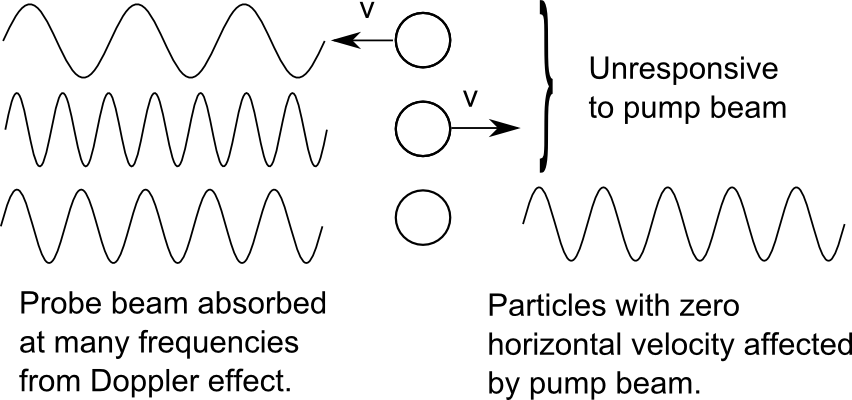
\includegraphics[width=9cm]{doppler.pdf}
    \caption{Doppler effect demonstration.  Probe beam is absorbed across a wide frequency range, but only the non-Doppler-shifted particles are affected by both beams from left and right.}
    \label{fig:doppler}
\end{figure}



%%%%%%%%%%%%%%%% BACKGROUND THEORY / PROPOSED METHOD

\newpage
\section{Theory and Implementation} \label{sec:theory}

To gain an understanding of the motivations behind this project it is worthwhile to discuss both prior work done with the PDH method, and the motivations behind using it to lock to an atomic source.  The PDH method is often used to lock a laser to an actuated cavity \cite{black1998}.  The Madison group primarily performs laser cooling experiments on Lithium and Rubidium gas.  They need to precisely set laser frequencies at or near key atomic transitions. For example, the Rb87 $5S_{1/2} \rightarrow 5P_{3/2}$ or "D2" transition is the focus of this project.  The closer a laser's frequency is to a desired transition and the smaller the linewidth of that laser, the more efficient any excitation will be.  This has a direct impact on experimental outcome.

\subsection{Brief Overview of Saturated Absorption Spectra}

Using a vapour cell as a frequency selective feature means that the error signal
is being generated from the absorption absorption spectrum of the particular
vapour. To understand what this spectrum looks like, it is sufficient to do a
basic analysis using semi-classical derivations. Because the gas is not
collimated, and is sufficiently hot (room temperature), the constituent
atoms are moving in every direction with the typical Maxwell-Boltzmann speed
distribution. As the primary concern is exposure to a laser beam, the
velocity classes to be considered here are distributed in one direction only,
here referred to as "z":
\begin{gather}
  \rho(v_z) = \sqrt{\frac{m}{2\pi k_B T}} e^{\frac{-m v_z^2}{2k_B T}}
\end{gather}
Each velocity class absorbs the incident beam at a rate that is dependent on
how far it is from a transition resonance. Furthermore, if the atoms are not
stationary, then the incident light is Doppler shifted. This results in the
standard Lorentzian absorption profile with a Doppler correction:
\begin{gather}
  F(\nu, v_z) = \frac{\Gamma / 2 \pi}{(\nu - \nu_0 + \nu_0 v / c)^2 +
  \Gamma^2 / 4}
\end{gather}
where $\nu_0$ is the transition resonance, and $\Gamma$ is the transition
linewidth. Putting these two terms together, and integrating over all velocity
classes in the "z" direction results in a term known as \emph{optical depth}:
\begin{gather}
  \tau(\nu) = \int_{-\infty}^\infty F(\nu, v_z) \rho(v_z) dv_z
\end{gather}
which is a measure of the sample's tendency to absorb an incident photon of
frequency $\nu$. \\

An incident laser beam will enter the vapour cell and be absorbed according to
the optical depth of the medium. However, photons will be re-emitted in a random
direction and so the intensity of the incident beam will be attenuated in the
original propagation direction, depending on its frequency and the quantity
of the medium it has passed through:
\begin{gather}
  I(\nu, z) = I_0 e^{-\tau(\nu)\cdot z}
\end{gather}
Plotting $I/I_0 (\nu, L)$, for some fixed vapour cell length L, and for
values corresponding to the Rb87 D2 transition generates a
a fairly broad absorption spectrum that is essentially Gaussian with a width of approximately 1GHz \cite{maguire2006}.  Using the PDH method to lock to this feature
alone is not atttractive as it generates a very low slope about the null locking
point. If a laser is needed to specifically excite a particular hyperfine
transition, for example, this locking method will not be sufficient. \\

To generate a feature which is suitable for tight locking, a profile known as a
saturated absorption spectrum is generated by exciting the vapour cell with
a beam propagating in the opposite direction of the master laser beam. This beam
is referred to as the "pump" beam, as it serves to pump some of the atomic
population into the excited state and make it innaccesible to the original beam,
hereby referred to as the "probe". The pump beam is normally derived from the
probe beam itself. This results in an additional effect that starves the probe
beam of accessible atoms. For a simple two level system, this can be written as:
\begin{gather}
  S(I_p, \nu, v) = \tau_0 \frac{\nu_0}{c} (P_1 - P_2) =
    \tau_0 \frac{\nu_0}{c} (1 - 2 P_2)
\end{gather}
where $P_1$ and $P_2$ are the ground and excited state population, respectively,
and the other terms are simply normalization constants. An expression for
$P_2$ can be derived that depends on the pump beam intensity, $I_p$, frequency,
$\nu$, here the same as the probe, and the linewidth of the transition
\cite{maguire2006}:
\begin{gather}
  P_2(I_p, \nu, v) = \frac{ (I_p/I_{sat})/2}{1 + (I_p/I_{sat}) +
    4(\nu - \nu_0 - \nu_0 v/c)^2/\Gamma^2}
\end{gather}
Implementing this factor into the prior calculation gives a corrected optical
depth:
\begin{gather}\label{eq:corr_opt_depth}
  \tau'(\nu) = \int_{-\infty}^\infty S(I_p, \nu) F(\nu, v_z) \rho(v_z) dv_z
\end{gather}
The resultant saturated spectrum is shown in \textbf{Figure~\ref{fig:rb87d2abs}}
, for a variety of $I_p$. The emergent feature at the transition resonance is
referred to as a "Doppler-free" feature. This nomenclature refers to the fact
that the velocity class that is most exposed to both the pump and probe beam
is the class around $v_z = 0$. This results in a decrease in probe beam
absorption from that class, and therefore, a higher transmission ratio.
This feature is shown in more detail in \textbf{Figure~\ref{fig:rb87d2abs_closer}}.

\begin{figure}
  \centering
  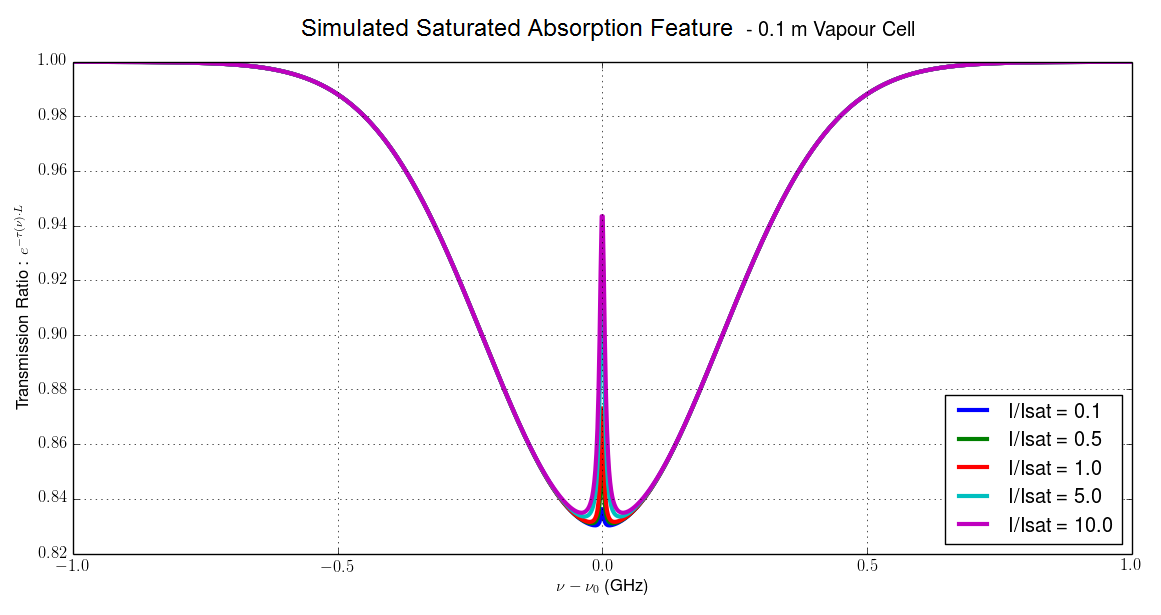
\includegraphics[scale=0.5]{rb_D2_single_absorption.png}
  \caption{Transmission ratio of probe beam through a 0.1m long cell of Rubidium
  gas, near the D2 feature. Optical depth is calculated as shown in
  \textbf{(\ref{eq:corr_opt_depth})},
  and all hyperfine splitting is ignored, (assumed 2-level system) for
  simplicity. The spectrum is plotted for a variety of pump beam intensities
  showing the saturating effect on the velocity classes near $v_z = 0$ at
  resonance.}
  \label{fig:rb87d2abs}
\end{figure}

\begin{figure}
  \centering
  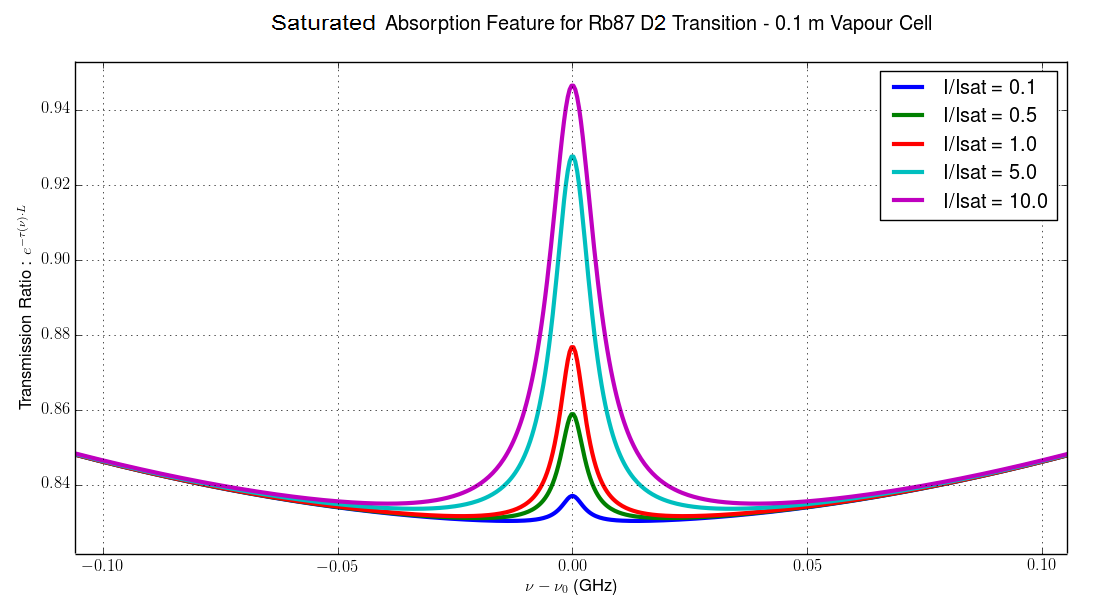
\includegraphics[scale=0.5]{rb_D2_single_absorption_resonance.png}
  \caption{Closer view of \textbf{Figure~\ref{fig:rb87d2abs}}, near the
  resonance.}
  \label{fig:rb87d2abs_closer}
\end{figure}

The model presented here is naive. The Rb87 $5P_{3/2}$ state has 4 hyperfine
levels, and transition from the ground state is goverened by the standard
selection criteria (\cite{steckrb87}, see Figure 2). This produces a much more
complicated absorption feature, with multiple transition and crossover
resonances (\cite{maguire2006}, see Figure 3). Calculating an optimal modulation
frequency for locking about one of the predominant resonance features inside the
Rb87 D2 spectrum can be done with detailed quantum mechanical analysis. It is
unclear if this is necessary, or whether the locking unit should simply be built
with an appropriate phase modulation bandwidth such that heuristic tuning can
attain an optimal result.

\subsection{Optical Phase Modulation}

As it is not possible to process optical signals in the THz range electronically,
it is common to modulate these signals to produce a spectrum about the carrier,
and then down-mix them to RF signals to extract the relevant information.
For optical signals, this is typically done with either an AOM or an EOM. From
a mathematical standpoint, the only difference between the two methods is
what phase modulation depths and frequencies are physically attainable. \\

With AOMs, which use acoustic waves to Doppler shift a beam in the transverse
direction of propagation, there is a distinct tradeoff between modulation
frequency and the resultant power of the outgoing beam.  The AOMs in current use by the Madison Group only have a useful
modulation frequency of approximately 200 kHz \cite{madison14}. \\

The modulation frequency of an EOM is sustainable well into the 100 MHz range,
with modulation depth a function of the driving voltage. Furthermore, as
phase modulation is parallel with the beam propagation, there is no significant
decrease in total beam power as the modulation frequency is increased. High modulation
frequencies do, however, result in higher electrical power consumption.
Typical modulation depths are in the 100mRad range, with a driving voltage of
$\sim 10 V_{pp}$ \cite{thorlabs_eom}. A higher modulation depth demands a higher driving voltage,
which also results in higher power consumption, which may or may not be of
concern. \\

The effect of the phase modulating medium is to induce a phase oscillation
in the incident laser:
\begin{gather}
  E = E_0 e^{i\omega t} \xrightarrow{Phase Modulation}
    E_0 e^{i \omega t + \beta \sin \Omega t}
\end{gather}
where $\beta$ is defined as the modulation depth, in radians, and $\Omega$ is the
modulation frequency. Using the Jacobi-Anger expansion to isolate the sideband
amplitudes,

\begin{gather}
  E_0 e^{i \omega t + \beta \sin \Omega t}  =
  E_0 e^{i\omega t} \sum_{n = -\infty}^{n = \infty} J_n(\beta)e^{in\Omega}
\end{gather}

it is shown that a sideband of frequency $(\omega +n\Omega)$ has amplitude
$J_n(\beta)$, the Bessel function of order $n$, evaluated at $\beta$, the
modulation depth. If the modulation depth is sufficiently small, the following
linear approximation can be made:

\begin{gather}
  E_0 e^{i \omega t + \beta \sin \Omega t}  \approx
    E_0 e^{i\omega t} \left(1 + \frac{\beta}{2}e^{i\Omega t} -
      \frac{\beta}{2} e^{-i\Omega t} \right)
\end{gather}

A visual description of this process is shown in
\textbf{Figure \ref{fig:eom_spectrum}}.
An inspection of Bessel function behaviour near the origin shows that
this approximation quickly becomes invalid for large modulation depths, and
that the carrier amplitude is not conserved. This phenomenon becomes important
when considering the response of a photosensor to the carrier and side-band
amplitudes. These must be tuned such that the signal power is above the noise
floor of the FO receiver, but below the saturation level.

\begin{figure}
  \centering
  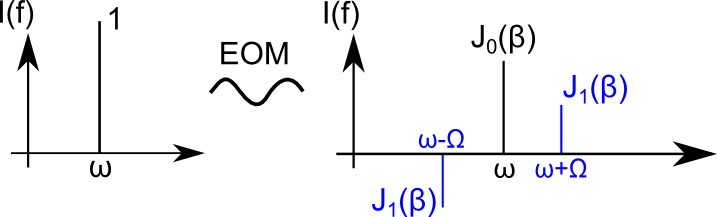
\includegraphics[scale=1.2]{spectrum.pdf}
  \caption{Expected spectrum of beam after phase modulation, to the first
  sidebands. While possibly present and significant, further sidebands can
  be ignored as they will be filtered during mixing.}
  \label{fig:eom_spectrum}
\end{figure}

\subsection{Error Signal Generation}

Obtaining an accurate value for the optimal error signal slope will be a central
development task, if it is not possible to obtain heuristically in
a way that is comfortable for the laboratory staff. Rigorous analysis will
involve some complex quantum mechanical models, but there are precedents for
reference \cite{maguire2006}. \\

The entire PDH error-signal generating setup is depicted in
\textbf{ Figure \ref{fig:setup}}.
The master laser enters at the left, and is immediately split by a
polarizing cube into two beams.  The lower "pump" beam (dashed line), unmodified,
reflects off of several mirrors, and is directed into a chamber full of
Rubidium gas. This beam serves to saturate the absorption ability of the gas,
which results in the a set of Doppler-cancelled features.
The most predominant of these features is used as a locking point. \\

The second "probe" beam is passed into an EOM.  This modulator is fed by a VCO,
running at frequency $\Omega$. As previously discussed, this creates the spectrum
shown in \textbf{Figure \ref{fig:eom_spectrum}}. After being passed through the
vapour cell, the amplitudes of the carrier and the sidebands are attenuated
according to the transmission profile of the saturated absorption feature,
of which a naive representation is shown in
\textbf{Figure \ref{fig:rb87d2abs}}. Let $\hat{F}$ be the operator that
describes the attentuation of the probe beam as it passes through the
vapour cell. Then, the resultant beam is, to the first sidebands:
\begin{gather}
  E_0 e^{i \omega t + \beta \sin \Omega t} \xrightarrow{\hat{F}}
    E_0e^{i \omega t }\left( J_0(\beta)\hat{F}(\omega) +
      J_1(\beta)\hat{F}(\omega + \Omega)e^{i\Omega t} +
        J_1(\beta)\hat{F}(\omega - \Omega)e^{-i\Omega t} \right)
\end{gather}

\begin{figure}
  \centering
  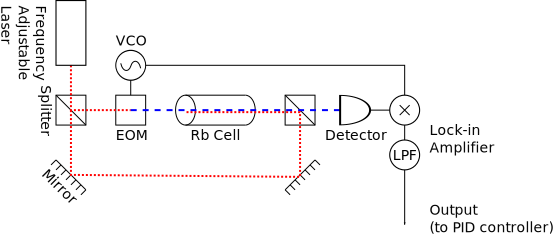
\includegraphics[scale=0.95]{setup.pdf}
  \caption{High level layout of the proposed PDH servo loop using a Rubidium
   vapour cell as the frequency selective element.}
    \label{fig:setup}
\end{figure}

This beam is then coupled into a high-speed fiber optic receiver, a
photosensor unit with bandwidth up to 12GHz. The current produced by the
biased sensor is proportional to the incident optical power. As
$P = |E|^2$, this creates a signal with some mixed frequency components. After
applying a low pass filter to this signal, with a pole at $\sim 1.5 \Omega$,
the following waveform is extracted:
\begin{gather}
  V_1(t) = A(\hat{F}, \omega, \Omega) E_0^2 +
    E_0^2 (J_0(\beta)J_1(\beta))
    (\hat{F}(\omega + \Omega) - \hat{F}(\omega - \Omega))cos(\Omega t)
\end{gather}

Where  $A(\hat{F}, \omega, \Omega)$ is some down-mixed DC term that is dependent
on carrier and side-band powers, as well as the frequency selective element
(it will be filtered out shortly). It is clear even at this stage, that being
able to isolate $(\hat{F}(\omega + \Omega) - \hat{F}(\omega - \Omega))$ will
provide some variable accuracy estimation of the \emph{derivative} of the
saturated absorption spectrum, and will provide a convenient null locking point
at any absorption peaks, which are located at important resonances. To extract
this value explicitly, $V_1$ is mixed with a phase delayed version of the
VCO signal, of frequency $\Omega$ and filtered to extract the DC error signal,
which is explicitly:
\begin{gather}\label{eq:err_sig}
  \epsilon = \alpha E_0^2 (J_0(\beta)J_1(\beta))
    (\hat{F}(\omega + \Omega) - \hat{F}(\omega - \Omega))\cos\phi
\end{gather}
where $\alpha$ is some attentuation factor, dependent on electrical components,
and $\phi$ is the phase delay between the oscillator signal being mixed
and the oscillator signal driving the EOM (same source, one passes through
extra cabling and other components such as buffers, etc). It is clear that
care must be taken to select an appropriate $\phi$ so as to generate a
clear, useable error signal. $\epsilon$ is then fed back into the
laser controller and used to sweep $\omega$ as necessary.
An example error signal, using the naive Rb87 D2 profile in
\textbf{Figure \ref{fig:rb87d2abs}} and generated with different phase modulation
frequencies to show the change in slope about the lock point is shown in
\textbf{Figure \ref{fig:err_gen}\subref*{fig:error_far}}, with an explicit
change in the slope made clear in
\textbf{Figure  \ref{fig:err_gen}\subref*{fig:error_close}}. It is clear from
this analysis that, for this particular absorption profile,
there exists some $\Omega$ between 100kHz and 10MHz that produces
the maximum error signal slope. Maximizing the slope is important as it provides
the smallest drift in frequency for a given change in signal voltage, which
allows any locking system to lock closer to the resonance, given a particular
voltage resolution. If the absorption spectrum for the Rb87 D2 transition has
similar feature size, then it is clear that the existing AOM solution is,
at best, suboptimal.

\begin{figure}
  \begin{tabularx}{\linewidth}{c}
    \subfloat[View far from the null lock point, showing the entire
    feature and generated error signals.]
    {
      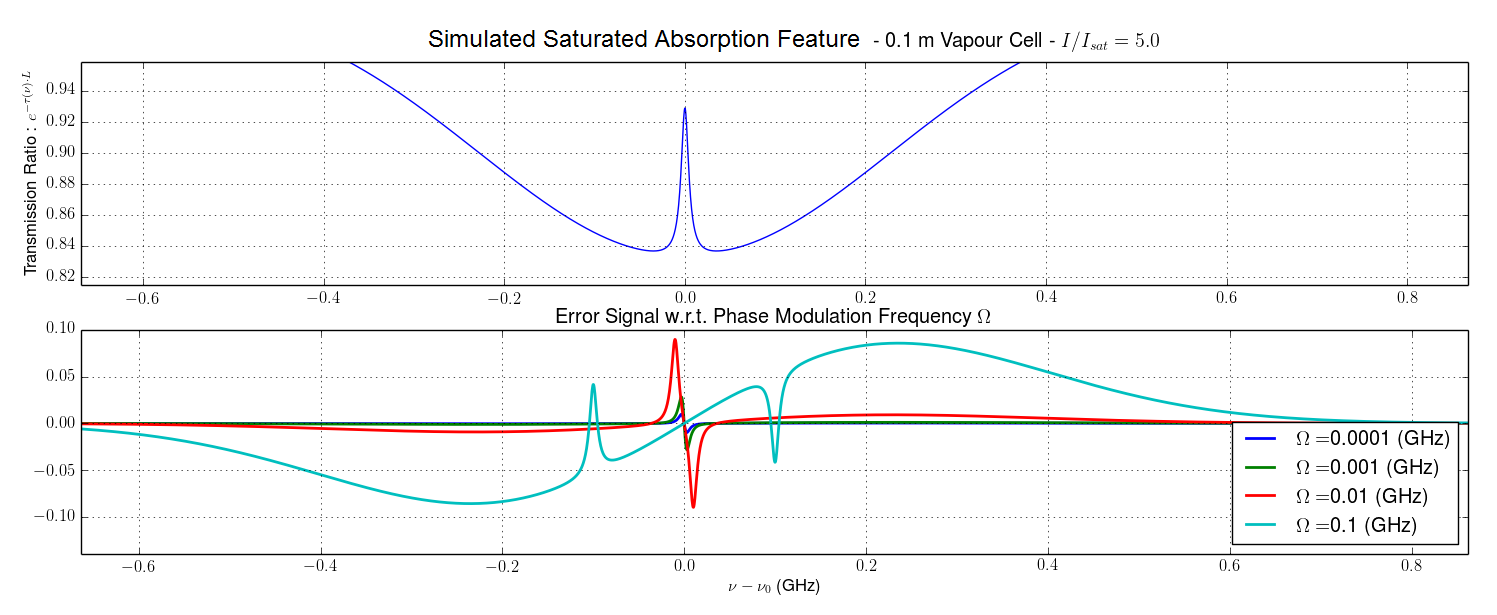
\includegraphics[height=0.5\linewidth, width=\linewidth]
        {rb_D2_error_faraway.png}
      \label{fig:error_far}
    } \\
    \subfloat[View close to the  null lock point, showing the change in
    slope about it as $\Omega$ is varied.]
    {
      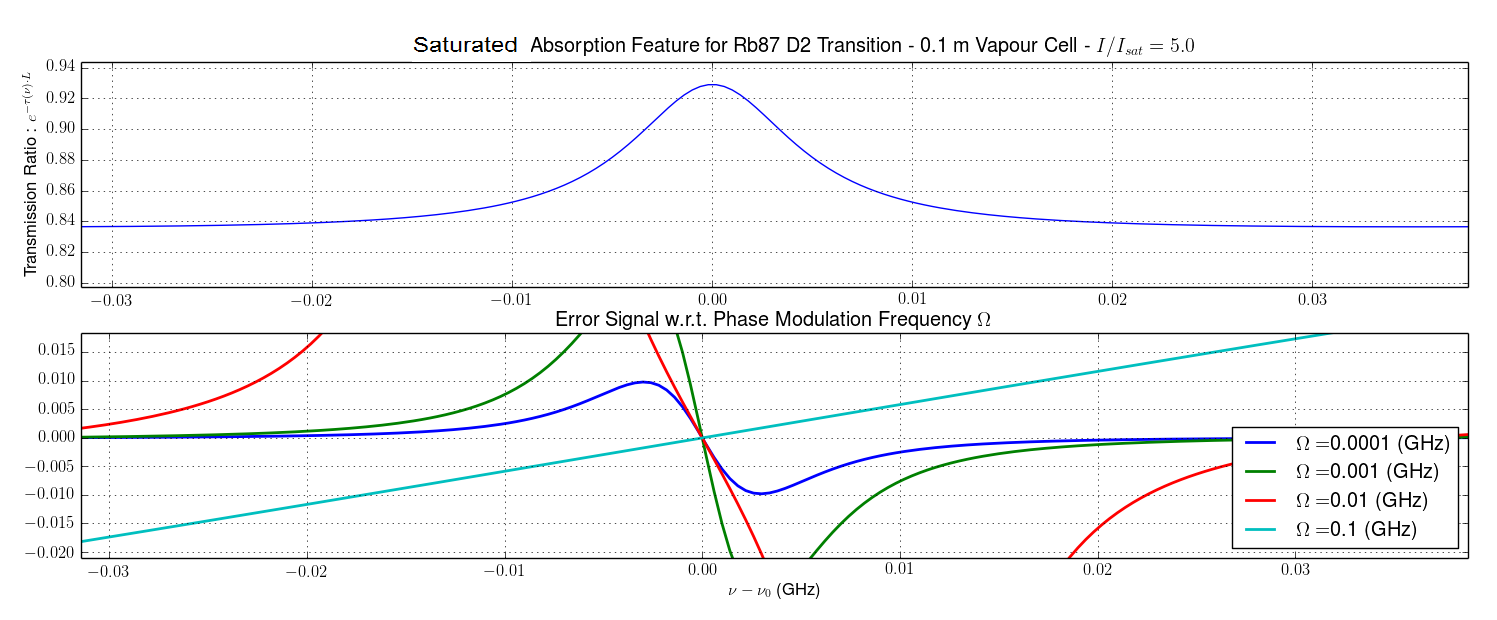
\includegraphics[height=0.5\linewidth, width=\linewidth]
        {rb_D2_error_closer.png}
      \label{fig:error_close}
    }
  \end{tabularx}
  \caption{Generation of an error signal with varying modulation frequencies
    / sideband separation $\Omega$, using (\ref{eq:err_sig}), for a
    saturated absorption feature generated with (\ref{eq:corr_opt_depth}).
    It is clear,
    especially in \protect\subref{fig:error_close}, that there is some
    optimal value for $\Omega$ that creates the largest slope about the
    null lock point. This value will be highly dependent on the size
    of locking features in the saturated absorption spectrum. }
  \label{fig:err_gen}
\end{figure}


%%%%%%%%%%%%%%%% DELIVERABLES

\newpage
\section{Deliverables}

%%%%%%%%%%%%%%%% PROJECT SCHEDULE / WORK PLAN / COMMUNICATION (subsections for the last 2)
%%%%%%%%%%%%%%%% MILESTONES
%%%%%%%%%%%%%%%% WORK/BUDGET/RESOURCES

\newpage
\section{Work Plan}

It should be noted that this project is quite complex in nature, and that
any estimates here are likely to change during development. Of particular
concern are any steps which require significant debugging or integration with
existing experimental instruments.

\subsection{Milestones} %%%%%%%%%%%%%%%%% MILESTONES

The following milestones have been tenatively agreed to by both sponsor and
team members.

\begin{enumerate}
  \item{\textbf{Principal Schematics, BOMs} - 2014-10-12}
  - Subunit schematics
  and block diagrams must be completed. Optical assembly schematics may be
  graphical (not a specific CAD format) but must be properly labeled and
  included with the relevant physical models referenced. Electrical schematics
  for any CCAs should be completed, reviewed and approved. All
  relevant BOMs should be compiled and be ready to order. Lead times should be
  minimized as much as possible (1-3 weeks maximum), as there are no
  anticipated long-lead components. In this time, the existing AOM locking
  circuit must also be benchmarked as discussed.
  \item{\textbf{Mechanical Design, PCBs Finalized} - 2014-10-31}
  - Lead times for PCBs have historically been no longer than 1-2 weeks. Should
  CCAs have to be designed
  for EOM control and signal mixing, time will be spent here doing actual PCB
  layout and designing mechanical enclosures, with cooling options, if
  necessary. At this milestone, all designs should be approved and ready to
  order or be in the process of being ordered.
  \item{\textbf{Principal Assembly} - 2014-11-21}  This milestone is for a
  fully \emph{assembled} servomechanism, with all optical, electro-optical and
  electrical assemblies built and ready for testing. During this time,
  basic electrical testing - ensuring zero short-circuit conditions and correct
  inter-net connectivity - should be complete, with specific functional testing
  to be completed later. All optical elements should be assembled on an optical
  breadboard and be roughly calibrated such that beam propagation is close to
  ideal.
  \item{\textbf{Final Unit Delivery} - 2014-12-14} Upon delivery, the
  new PDH unit should ideally be fully built, functionally verified and
  benchmarked against the existing solution. At this stage the units would be
  ready for use in experiments.
\end{enumerate}

\subsection{Task Schedule}  %%%%%%%%%%%%% SCHEDULE

The proposed milestone schedule is broken up into tasks ([Milestone\#-Task\#]).
These are estimates of work that must be completed and may be subject to
alteration. The specifics behind each of these tasks are as follows (with
completion time estimates in brackets):

\begin{packed_itemize}
  \item{\textbf{[1a] Completion and Approval of Physical Models} (24 hrs)}
  - This constitutes a well-formatted block diagram of every unit in the servo
  loop as well as associated physical models. The format of the error signal
  should be explicit and well defined with respect to physical parameters (
  actual equations). This model is to be used as a reference for physical
  design and must be approved by the sponsor. If mandated, time will be spent on
  fully developing the quantum mechanical saturated absorption profile to
  determine the optimal phase modulation frequency.
  \item{\textbf{[1b] Electrical Schematic*} (24 hrs)}
  - A controller CCA may have to be designed and built. At this stage,
  the electrical schematic, with all of the components necessary for controlling
  the EOM and mixing the error signal. This will consist of, at the very least
  a VCO up to 100MHz, a VCO controller (if needed), the lab computer digital
  interface and analog mixing circuits (to be deterimined).
  \item{\textbf{[1c] BOM compilation and Component Ordering} (12hrs)}
  - This is potentially a significant step if any CCAs are to be designed.
  Components will have to be sourced and the requisite invoices will have to be
  produced so that the Madison Lab can put an order through. Depending on the
  number of suppliers involved, this step may represent a significant amount of
  paperwork/communication, and is not inconsequential.
  \item{\textbf{[1d] Evaluation of Existing AOM Servo} (36 hrs)}
  - The existing AOM based PDH unit is to be benchmarked for parameters such as
  its noise floor and slope around the locking point, as well as the resulting
  linewidth of the master laser. These features can be evaluated with equipment
  in the Madison Group laboratory. Fiber coupled laser sources are readily
  accessible within the laboratory. However, it is unclear whether the PDH
  feedback unit in existance will be in use for ongoing experiments. If so,
  a separate unit will have to be quickly constructed. All of the components
  for this should be readily available wtihin the Madison Group laboratory.
  \item{\textbf{[2a] Mounting Hardware}} (12 hrs)
  - It is likely that some mounting hardware will have to be constructed for
  various controllers and optical units to sit in either a standard equipment
  rack or near electro-optical elements on an optical table. Whether the EOM
  driver or FO receiver can be coupled to with long coaxial cables or fiber is
  dependent on how much attenuation is tolerable.
  \item{\textbf{[2b] Possible Signal Processing / EOM Controller CCA*} (24 hrs)}
  - If it is not possible to construct the EOM driving and signal mixing
  electronics from a collection of discrete RF components, a custom PCB will
  be designed and assembled in-house. This will likely not take long, discounting
  any difficulties in the electrical design stage, as group members have
  significant experience with PCB construction and layout. In this stage, actual
  board layout will likely take less than 12 hours.
  \item{\textbf{[3a] Assembly of Optical Breadboard} (6 hrs)}
  - Once acquired, all optical and electro-optical components must be assembled
  on an optical breadboard. This is simply a plate of moderate size with a
  grid of threaded holes to fasten standard optical elements to. The equipment
  required for this is avilable in the Madison lab. This is not expected to
  be difficult, but it may take some time to carefully lay out.
  \item{\textbf{[3b] Soldering and Assembly of custom CCAs*} (6 hrs)}
  - Should any custom CCAs be required, time will be spent soldering their
  components and doing basic electrical testing to ensure no short-circuit
  conditions and correct inter-net connectivity, etc.
  \item{\textbf{[3c] Manufacture and Assembly of Cabling/Interconnects} (3 hrs)}
  - Cabling must be created for connecting to laboratory power supplies
  and powering various components. Manually fabricated cabling will likely be
  standard braided cable with various MOLEX connectors. Any high-speed
  (100MHz +) cabling will likely be pre-purchased to maintain quality.
  \item{\textbf{[3d] Final Comprehensive Assembly} (12 hrs)}
  - This stage involves integrating all previously assembled subunits into their
  laboratory configuration. This will involve placing the optical assembly,
  placing any controlling electronics, connecting these components and then
  integrating them with any test equipment or lab systems.
  \item{\textbf{[4a] Unit Block Validation} (12hrs)}
  - All subunits will be quickly tested to ensure that they produce signals that
  are at least qualitatively correct. This is considered the "trial run" as it
  will hopefully identify any major problems, such as overattenuation,
  excessive power draw, excessive noise or instability, etc. The servomechanism
  will be evaluated piecewise to ensure that component feedthrough is correct.
  \item{\textbf{[4b] Comprehensive Benchmarking} (24hrs)}
  - This step mirrors step [1d], but for the presumably-finished EOM-based
  locking unit. Identical parameters will be extracted, and compared with
  those of the AOM solution, to formally establish improvement metrics.
  \item{\textbf{[4c] Fine Tuning / Final Configuration} (???, 24hrs ++)}
  - With current background knowledge and understanding, it is not possible
  to predict how long tuning the system will take. While the scope and
  technical background behind the project is understoood, anticipating
  complications that may arise from problems such as component nonlinearities or
  induced noise is not currently possible. This is expected to be the
  longest single task of the project.
\end{packed_itemize}

Tasks marked with (*) are potentially unnecessary, should ready-made solutions
be found. The total estimated task time, barring final debugging, sums to 180
hours over the term. The testing and assembly estimates are likely accurate, as
they are based on previous experience. However it is likely that the model
development and testing will exceed the estimated time significantly as this
project is based on complex physical principles and has high technical demands.
The final debugging step is estimated to take the most amount of time and effort
as there is potential for significant problems to arise. Fixing these problems
will require some re-design and re-assembly, followed by further testing. This
testing, in particular, has the potential to take a long time, especially if
significant lab resources are required.

\subsection{Team Responsibilities} %%%%%%% RESPONSIBILITY

As per the proposal guidelines, the following team members are assigned the
suggested team roles:
\begin{packed_itemize}
  \item{\textbf{Steve Novakov} - Project Manager}
    \begin{packed_itemize}
      \item shall maintain and ensure project schedule
      \item shall submit proposal and recommendation report and delegate their
      workload
      \item shall maintain communications with sponsor and schedule meetings,
      when necessary
    \end{packed_itemize}
  \item{\textbf{Jeff Taylor} - Technical Manager}
    \begin{packed_itemize}
      \item shall submit weekly reports and maintain project technical data
      \item shall drive testing and validation efforts
    \end{packed_itemize}
\end{packed_itemize}

The nature of the project is such that both members shall be conducting
investigations and driving design schedules, but the roles are explicitly
delegated for formality, with the designated members having final oversight
and providing approval. The sponsor shall interact with both team members on a
regular basis making the single liason role meaningless.

\subsection{Sponsor Interactions}  %%%%%%% SPONSOR INTERACTIONS

With respect to communicating with the sponsor, Dr. Kirk Madison, there shall
at least be one weekly email sent every Wednesday night summarizing work that has
been completed and upcoming tasks in a relevant timeframe. These shall mirror
the content of the weekly 479 reports, but will be composed with the sponsor in
mind (more specifics, more technical jargon). During any stages where there
is a need for interaction with Madison Group laboratory equipment, (e.g. during
testing and benchmarking, the appropriate lab staff, likely a graduate
student or Dr. Madison himself, shall be consulted with to approve and possibly
assist with the procedure.

\subsection{Resources and Budget}

At this time, it is possible to identify several high-level items (with lack of
specificity about sub-assemblies) which will be necessary to construct the PDH
unit. These items, with some commentary on status and price,
can be reviewed in \textbf{Table \ref{budget_table}}

\begin{table}[!hrt]
  \begin{tabularx}{\linewidth}{|L|L|L|}
  \hline
  \textbf{Item} & \textbf{Status} & \textbf{Approx. Purchase Cost (source)} \\
  \hline
  Rubidium Vapour Cell & exists in inventory & \$500 (Thorlabs) \\
  EO Phase Modulator & exists in inventory & \$2,500 (Thorlabs) \\
  High-speed FO Receiver & exists in inventory & \$200 (custom) \\
  PDH Controller CCA & as necessary & $>$\$200 (custom) \\
  Discrete RF Compoonents & as necessary &$>$\$200 (Mini-Circuits) \\
  Cabling and Accessories & as necessary &$>$\$200 (Mini-Circuits) \\
  \hline
  \end{tabularx}
  \caption{Brief overview of major subcomponents and their estimated status,
  with respect to acquisition. Items stated to "exist in inventory" are likely
  available for use from the Madison Lab, but are allowed to be purchased, if
  necessary. Price estimates may represent an amalgamation of
  components from various vendors.}
  \label{budget_table}
\end{table}

There is no established hard limit on the budget for this project, but, as all
purchases must be approved by Dr. Madison, they are expected to be provably
reasonable and necessary. For example, should a new EOM unit need to be
purchased, it may cost anywhere in the neighbourhood of \$2000-3000. With respect
to the PDH Controller CCA, which must be designed and built sometime this
term, the board and components will likely price in the \$200-300 range.
The Madison Group does have many optical components and optical breadboards
in storage and available for use. It is unlikely that any optics will have to
be purchased, again, unless provably necessary. It is possible that some
mounting hardware will have to be purchased or manufactured, but there is
allowance for small work jobs to be done by the UBC Hennings machine shop,
if necessary. Fiber optic receivers, with bandwidth up to 12 GHz are readily
available throughout the laboratory.


%%%%%%%%%%%%%%%% RISKS / CONTINGENCY

\newpage
\section{Risks and Contingency}

Though the premise of this project, an increased-fidelity PDH error-signal
generator, may seem straightforward, there are several nuances which may
complicate development. The models presented in \textbf{Section
\ref{sec:theory}} are meant to give a qualitative overview of why this upgrade
is justified, but they ignore or simplify many parameters.

The signal processing here is mostly considered with the assumption that all
mixing or amplification is linear, and that signal attenuation, if present,
is minimal. In reality, the propagation of the beat-note signals through the
processing electronics may be more complex, with saturation effects and other
nonlinearities coming into effect. The incident side-band beat-note signals,
for example, may be subject to saturation effects in the phototransistor
depending on the incident laser power. This, and other effects, will have to be
carefully accounted for during electrical design. If something is overlooked,
it may be that tuning the locking unit is more difficult than anticipated.

As mentioned, another point of contention is the operation of the EOM unit
itself. Choosing between a readily-available but small-bandwidth low-power EOM
which is tuned around some built-in fixed-bandwidth amplifier, or developing
a custom high-power, wide-bandwidth driver will vastly change the amount of
work that must be done to arrive at a functional unit. Time spent designing an
EOM controller, estimated to take 1-2 weeks, would alternatively be used on
assembly and benchmarking. Making use of a pre-configured EOM would be ideal, but
if the error signal generated by its modulation frequency is less-than-ideal,
analysis and testing of alternative solutions will have to take place.
Implementing the full quantum mechanical description of the Rb87 D2 absorption
spectrum will allow for direct derivation of an optimal modulation frequency.
However this process would likely take the better part of 2-3 weeks, requiring
substantial modelling, simulation and consultation with the sponsor. Having a
ready-made unit perform adequately, but not optimally, is still ideal because
more time can be spent on final debugging, characterization and integration.

The primary detractor to how complete this project will be at delivery
is the amount of custom solutions (CCAs, custom software, etc) that must be
built in-house. Presumably, if the entire control loop can be built from
off-the-shelf components from, for example, Thorlabs and Mini-Circuits,
then a significant amount of time will be devoted to fine-tuning and
benchmarking a ready-to-use assembly. The sponsor has requested two functional,
benchmarked PDH reference units at project completion. It is inconcievable that
these units will not be, at the very least, fully built during this term. Lack
of built PDH reference units, consisting of the opto-electronic assembly and
electronic mixing components, by 2014-12-20 is considered a project failure.
The sponsor has allowed for testing and benchmarking to be completed after
delivery, if absolutely necessary.

%%%%%%%%%%%%%%%% CONCLUSION

\newpage
\section{Conclusion}

The UBC Quantum Degenerate Gases Laboratory is currently using an acousto-optic modulator-based system to lock a diode laser to a specific frequency.  This system is frequency limited, and is incapable of providing the narrow linewidths that they require for their experiments. \\

\section*{Acknowledgements}
\addcontentsline{toc}{section}{Acknowledgements}

This project was aided immensely by the research staff in the UBC Quantum Degenerate Gases laboratory led by Dr. Kirk Madison. Dr. Madison provided direct guidence on theoretical matters and contributed significant physical resources. Gene Polovy and Will Gunton of the Madison Group were extremely helpful with the physical setup, and with locating equipment. Janelle van Dongen provided significant assistance with the laser control instrumentation and data acquisition. Further thanks goes to Dr. David Jones, Dr. Jim Booth, Mariusz Semczuk, Koko Yu, Kahan Dare and Kais Jooya for their suggestions and guidance.

%%%%%%%%%%%%%%%% REFERENCES

\newpage
\printbibliography

\end{document}



